% \cleardoublepage
\chapter{Introduction}
\minitoc\label{sec:introduction}\vspace{.5cm}

\section{Background and Motivation}
A physical tunnel allows vehicles to move between 2 places independently from surrounding geography. 
Similarly, network tunneling is a mean to organize traffic between host A and B in a way that:

\begin{itemize}
    \item Abstracts the underlying path over the public network: Applications binding to the tunnel are not aware of the real paths that packets take.
    \item Encapsulates and encrypts the traffic: Man in the middle attack can't always determine if a network frame belongs to the tunnel or a tunnel is being used, nor decrypt the content.
\end{itemize}

% A \ac{VPN} is a application build on top of a tunnel to connect 2 networks, effectively allow its host to access the other internal network remotely.
% Well known \ac{VPN} applications can be named: \ac{wgpage}, \ac{ovpnpage}, IPsec, PPTP, PPPoE, L2TP, ...
% Despite of the difference in level of operation (network or data link layer) and operation space (kernel or user space), they generally share the same concept of single link: the tunnel utilizes one single network link to transmit and receive the tunnel packets. 
A \ac{VPN} is an application that utilizes a tunnel to enable remote access to an internal network. 
Notable \ac{VPN} applications include \ac{wgpage}, \ac{ovpnpage}, IPsec, PPTP, PPPoE, L2TP, and more. 
Despite variations in their operational level (network or data link layer) and operation space (kernel or user space), these applications generally share the concept of using a single link for transmitting and receiving tunnel packets.
% The connection with support for \textit{multipath} concept, would deploy multiple network links so it can achieve higher reliability through redundancy or higher bandwidth through combining links, even though these characteristics are more relevant to environment such as infrastructure, data center or industrial application rather than end-user usage.
% There are protocols such as \ac{MPTCP}, \ac{SCTP} work this way, albeit in form of non-sharable connection.
% A non-share connection is initiated similarly to initiating a socket and can only be used by the caller program. 
% This severely limits the capability to control, schedule and share multipath resources between multiple applications in an effective manner, i.e prioritizing, buffering ... 
% These require centralized orchestration level of control over all communication channels by a control plane, which doesn't exist for these protocols.
A connection that supports the concept of \textit{multipath} utilizes multiple network links to enhance reliability through redundancy or increase bandwidth by combining links. 
% However, these characteristics are more applicable to environments such as infrastructure, data centers, or industrial applications rather than regular end-user usage. 
Protocols like \ac{MPTCP} and \ac{SCTP} operate in this manner, but they are implemented as non-sharable connections and can only be utilized by the program initiating it. 
This limitation restricts the ability to effectively control, schedule, and share multipath resources among multiple applications. 
For instance, support for multiple flows with different quality of service requirements and priorities becomes challenging without a centralized control plane, which is currently absent in these protocols.\todo{review needed}
\\

We propose another tunnel implementation: \ac{MTX}. 
% The tunnel will have multipath support by design, allow multiple applications to share the connection simultaneously, and be built based on Linux's \ac{xdppage} socket family.
% Using the latest native Linux's technology, the implementation is expected to performance-wise outperform any user space implementation while retain compatibility with existing systems and code base's simplicity. 
% Support for multiple connection links offers reliability, large raw-bandwidth and a rich set of configuration to applications binding to the tunnel, makes it suitable for high demand use-cases such as industry, data center, telecommunication hub. 
% In this document, an enhancement for the 5G's \ac{gptu} protocol \todo{cut this} with \ac{MTX} library will be investigated. \ac{gptu} is the protocol that helps UPF and gNodeB functions of a 5G system communicating, which demands both bandwidth and stability and therefore is a suitable match for a \ac{MTX} demonstration.
The tunnel is designed to support multipath capabilities and allow multiple applications to concurrently share the connection. 
It is constructed based on Linux's \ac{xdppage} socket family, leveraging the latest native Linux technology. 
This implementation is expected to outperform user space implementations in terms of performance while maintaining compatibility with existing systems and ensuring simplicity in the code base.
The support for multiple connection links offers reliability, high raw-bandwidth, and a comprehensive configuration set for applications bound to the tunnel that is well-suited for demanding use cases such as industry, data centers, and telecommunication hubs.
For the experiment purpose, an enhancement for the 5G's \ac{gptu} protocol using the \ac{MTX} library will be investigated and developed. 
The \ac{gptu} protocol is an appropriate match for demonstrating the capabilities of the \ac{MTX} system since it facilitates communication between the UPF and gNodeB functions in a 5G system (\Cref{fig:introduction:3gpp_5g_data_plane_protocol}), demanding both bandwidth and stability.
\todo{review needed}
% The \ac{gptu} protocol facilitates communication between the UPF and gNodeB functions in a 5G system, demanding both bandwidth and stability. 
% Therefore, it is an appropriate match for demonstrating the capabilities of the \ac{MTX} system. \todo{improve}
%

\begin{figure}[H]
	\centering
	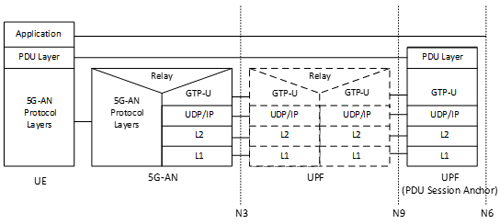
\includegraphics[width=0.8\textwidth]{resources/images/3gpp_5g_data_plane_protocol.png}
	\caption{3GPPP's 5G Data Plane protocol stack \cite{3gpp_5g_system_overview}}
    \label{fig:introduction:3gpp_5g_data_plane_protocol}
\end{figure}


% While it is possible to establish a connection between two applications using a single link, improving the bandwidth and reliability to support high-demand applications is a challenging endeavor. 
% In \Cref{sec:introduction:problem_statement}, we will outline the difficulties inherent in the current single-link methods and explore how the multipath approach can effectively tackle these issues.

\section{Problem Statement}\index{Requirements}\label{sec:introduction:problem_statement}
While it is possible to establish a connection between two applications using a single link, improving the bandwidth and reliability to support high-demand applications is a challenging endeavor. 
Currently, Ethernet and InfiniBand are the most prevalent communication technologies in data centers and \ac{HPC} environments (\Cref{fig:introduction:Interconnect_Technologies_500_supercomp}) which offer a line capacity ranging from 100-200Gb/s \cite{ethernet_roadmap}\cite{infiniband_roadmap}. 
While this bandwidth is impressive for inter-system communication, it cannot match the internal connections within a system. 
For instance, AMD's "Infinity Fabric" bridge offers an in-package bandwidth of 256GB/s on Zeppelin SoC family \cite{burd_zeppelin_2019}, and up to 800GB/s in peer-to-peer tests between GPUs using more bands \cite{amd_infinity_architecture}.
This indicates that the connection between computer instances can become a bottleneck for distributed data-intensive applications, for instance large \ac{AI} models or computer simulations. 
In such cases, a multipath tunnel can provides an abstracted connection, which hides the lines combination details from the application and thus effectively scales up the network capacity horizontally.
% In such cases, a multipath tunnel can take over the complexity of merging multiple links and exposed only the combined connection to the applications, effectively scaling up the network capacity horizontally. 
This way, a larger combined bandwidth can be formed using current technology and serves as a necessary tool to overcome future physical and economic limitations. \todo{review needed}

\begin{figure}[H]
	\centering
	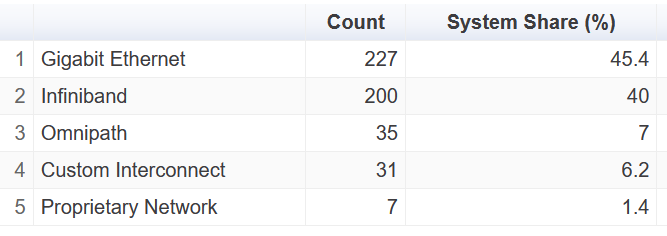
\includegraphics[width=0.8\textwidth]{resources/images/Interconnect_Technologies_500_supercomp.PNG}
	\caption{Interconnect technologies of top 500 super computers, 2023 edition as tracked by TOP500 project \cite{Interconnect_Technologies_500_supercomp}. Ethernet and Infiniband are the primary network technologies utilized in most systems.}
    \label{fig:introduction:Interconnect_Technologies_500_supercomp}
\end{figure}

The reliability of a connection is closely tied to the failure probabilities of the individual links and nodes, which directly impacts service availability \cite{shooman_algorithms_1995}. 
Additionally, \ac{QoS} of many applications is affected by network parameters such as latency, peak throughput, and jitter \cite{gozdecki_quality_2003}.
Depending on the use case, connection reliability can either serve as a \ac{QoS} measurement factor (e.g., for commercial network providers) or a strict requirement (critical applications). 
It is commonly acknowledged that ensuring a 99.99 percent reliability comes with a significant price tag, and pushing for such guarantees futher will likely result in an exponential cost escalation.
\\

Generally, there are two non-exclusive strategies commonly employed to enhance connection reliability: strengthening individual links or incorporating redundancy.
While superior hardware can reduce the probability of connection failures and address many \ac{QoS} inadequacies, having multiple links or routes optimized for specific applications is often a more practical and cost-effective approach for operators, particularly when dealing with heterogeneous data traffic \cite{chen_overview_1998}.
In such cases, a multipath tunnel with flow-aware capabilities can be utilized as an abstraction layer to manage the underlying links for applications relying on the connection, which allows for improved reliability and more effective utilization of resources. 
\todo{review}

% Perf: userspace vs kernelspace process
% Omitting trivial tasks such as authentication and handshake, tunneling operation including the following steps: acquiration of ingress data stream (send to tunnel by application), process of ingress data (convert data into stream of tunnel packets, often through encapsulating with tunnel header, encrypting, compressing), and reverse on the receiving end (extrating original data from tunnel packets and delivering to application) \todo{cite+improve}.
% Apart from scaling the underlying system vertically (i.e by using more powerful hardware) or using a lower-level programing language, the most significant factor that could affect the performance of a single-link tunnel implementation is how ingress data is handled.


\section{Assumptions and Scope}
The MTX project is inspired by \ac{5G}'s \ac{NFV} and \ac{SDN} influenced specification.
Being recognized as the two technology enablers for realizing 5G networks, they allow concepts such as \textit{slicing} or \textit{decoupling} \cite{yousaf_nfv_sdn_key_techno_for_5g2017} \cite{open_baton}, which make \ac{5G} a much more capable network standard than its predecessor while remains flexible and agile for operators.
\ac{NFV} moves dedicated functions such as router, firewall that traditionally ran on dedicated hardware to virtualized environment and cloud-based infrastructure.
\ac{SDN} encourages using software based solution running on common hardware and software stack over conventional equipments and services, which often integrated on rigid hardware-based proprietary.
\ac{NFV} and \ac{SDN} thus help reducing capital and operational expenditures, speeding up the release process and avoid vendor locking \cite{sun_integrating_2015}\cite{yousaf_nfv_sdn_key_techno_for_5g2017}.
These trends heavily influence the 5G infrastructure to employ recent software industry's practices, including Continous Integration/Delivery, orchestration, utilization of cloud, dynamic deployment, and \ac{HA} through horizontal partition.
This resulted in a distributed infrastructure that requires reliable and high throughput connection, which as discussed in \Cref{sec:introduction:problem_statement}, can be horizontally implemented in an performant and cost-effective way using a multipath tunnel. \todo{review needed}
% \ac{5G}'s distributed network services and diverse \ac{QoS} require reliable and high throughput connection, which as discussed in \Cref{sec:introduction:problem_statement} can be horizontally implemented in an performant and cost-effective way using multiple links instead of vertical scaling paradigm.
\\

% building block:
Moving functions to cloud and virtual environment faces performance challenges, one of which is the overhead introduced by the abstraction, virtualization layers as well as the extra input/output and communication between functions \cite{yousaf_nfv_sdn_key_techno_for_5g2017}.
Although running cloud-native software on thin, orchestrated containers help addressing the performance problem, we believe the connection can be improved further on some aspects, namely compatibility and ease of development and deployment.
This is because in many 5G's implementation, technologies such as \ac{dpdkpage} and \ac{sriov} are being used to deliver line-speed packet processing capability to hypervisor environment with minimal impact on system performance \cite{intel_dpdk_perf}\cite{nec_hite_paper_upf_perf}\cite{openstack_sriov}\cite{zte_5g_core_upf_impl}.
These technologies suffer from special requirement and configuration - in other words the commercial components are tailored picked and built for the purpose.
This would not only increase cost and decrease flexibility, but also make the product less attractive for purposes such as research and test bed, especially in the open source and academy community where budget and custom support is limited.
To address this, using a native and more simple Linux's technology - \ac{xdppage}, a new socket family based on eBPF technology with comparable performance to \ac{dpdkpage} - to build a tunnel that is designed to support multipath and multi-flow could be a promising supplement for existing implementation. \todo{review needed}
\\

% With an implementation and a thesis documentation for the multipath tunnel as the desire outcome of the project , we define the scope of the project as followed:
To overcome the limitations described, this work proposes MTX as an implementation for the multipath tunnel concept.
The scope of the project is defined as follows:
\begin{itemize}
    \item Scope of research: this research is limited to investigating a tunnel implementation based on \ac{xdppage} technology that employs multipath and flow-aware concepts. 
    A functional tunnel will be built in four months.
    A benchmark will be caried out.
    % From there, more complex features will be added along with a test application to run on top the tunnel for testing and demonstrating purposes. In the course of building process, this initiated documentation will be updated until the project reaches its time limitation (6 months in total). Although the tunnel library will be a general purpose framework that can be deployed for any application, it is intended to be tested with 5G's software stack in mind.
    \item Implementation: the tunnel will be implemented in C/C++ and uses \ac{xdppage} sockets as the packet transport layer. 
    The tunnel shall be able to exchange data over multiple \ac{NIC}s and treat each packet differently based on configuration (stream based/flow based). 
    More will be discussed in the next sections.
    \item Demonstration: for testing and presenting the features of the tunnel. 
    At current stage, a simplified version of \ac{gptu} protocol has been chosen as the application to run on top of the tunnel. 
    \ac{gptu} is the communication protocol responsible for establishing data exchanging channels in 5G's \ac{UPF} and gNodeB. 
    These channels (or tunnels) handle streams of data, each has \ac{QoS} identifier with different characteristics and priority. This makes the protocol a good match for tunnel demonstration purpose.
    \item Plan: the thesis is to be completed in 6 months. \Cref{sec:plan} will present the plan in details.
\end{itemize}

\begin{figure}[H]
	\centering
	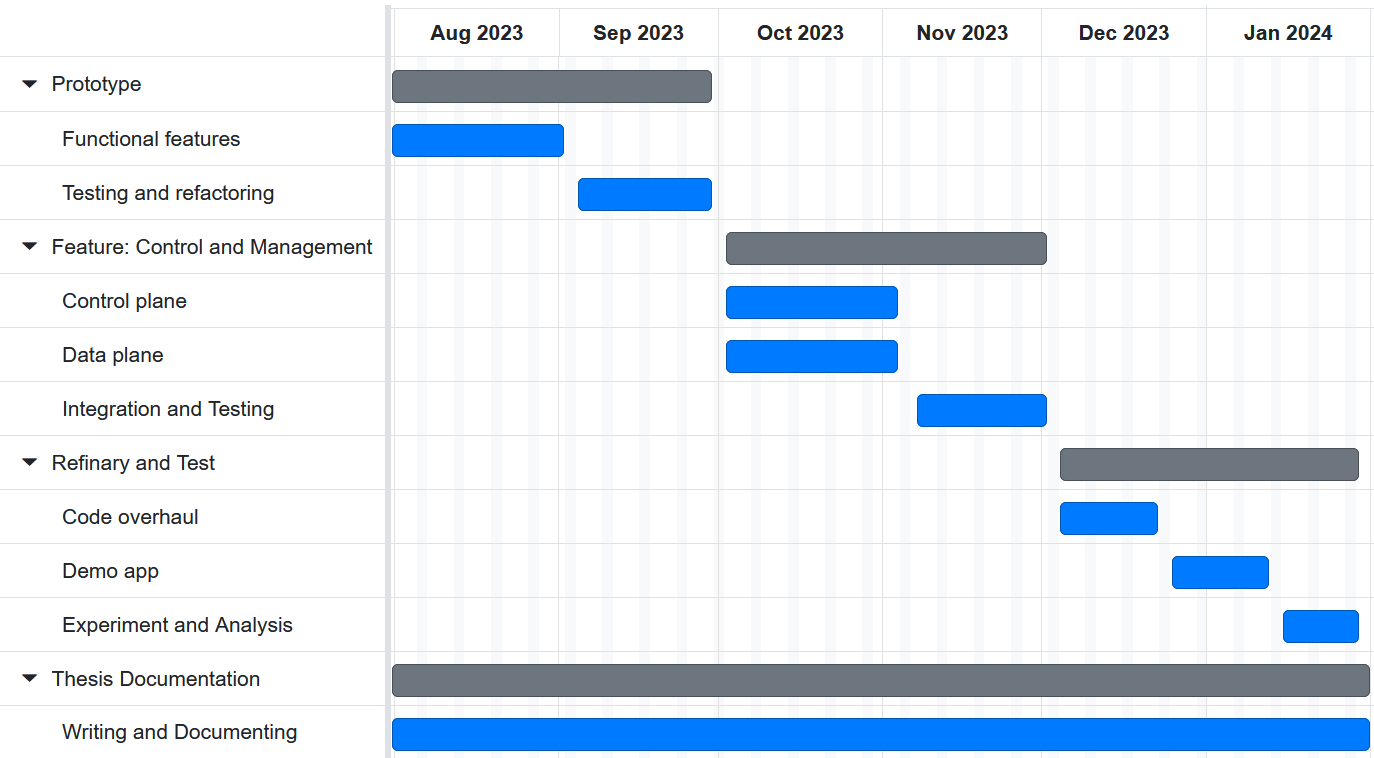
\includegraphics[width=1.0\textwidth]{resources/images/mini_gannt.PNG}
	\caption{Overview of the process to complete the thesis}
    \label{fig:introduction:mini_gannt}
\end{figure}

\section{Objectives and Contributions}
The main objectives of the project is defined as follows:
\begin{itemize}
    \item Multipath protocol design: Creating a well-defined header structure and establishing logic for traffic aggregation and distribution within the tunnel.
    \item Tunnel library: Create the MTX library that are capable of handling distributing and aggregating traffic over multiple lines for multiple applications simultainously. 
    Additionally, make configuration available to govern traffic on flow and packet levels.
    \item Implementation and packaging: The library will be developed in C/C++ programming languages for Linux system.
    \item Demonstration: Ideally, an implementation of the GPT-U protocol will be built to showcase the features of the tunnel.
\end{itemize}

The project contributes to the general understanding of software based solution for high performance networking field.
For practical application, reports regarding performance issues has been identified in the \ac{UPF} function of \ac{o5gs} - a well-known 5G core implementation that the AV team at the TU Berlin is currently using in their 5G test bed. 
Contributors have proposed employing \ac{dpdkpage} and exploring lower-level approaches to minimize overhead \cite{open5gs_github_udp_perf_cap}\cite{open5gs_github_dpdk}, as the current implementation limits the TUN interface bandwidth to 1Gbit. 
After through thorough analysis, this presents an opportunity to make a valuable contribution to the \ac{o5gs} project with the MTX tunnel.

%%%%
% Although we hope the project's outcome can contribute to the general understanding of software based solution for high performance networking field, we seek opportunity to integrate the tunnel into the next generation telecommunication system. We found 2 potential improvements according to our research: \todo{improve the following text}
% \begin{itemize}
%     \item N6 connection between UPF (also N9 i.e between UPF-E and UPF-C) and Data network: enhanced by prioritized, flow-aware, high bandwidth multipath tunnel. To meet differentiated SLA requirements for latency, bandwidth and reliability, UPF needs to be deployed at different positions including central DC, regional DC, edge DC and campus DC. MTX can help saturating physical links coup with support large number of UEs.
%     \item 5G user plane. The back-haul N3 connection between gNodeB-UPF, and mid-haul F1 connection between gNodeB-CU and -DU relied on message-based protocol \ac{gptu} (the character "U" means "user data tunneling") to relay traffic within a PDP session.
% \end{itemize}

% We also identified reports regarding performance issues in the \ac{UPF} of \ac{o5gs} - a well-known 5G core implementation that the AV team at the TU Berlin is currently using in their 5G test bed. 
% Contributors have proposed employing \ac{dpdkpage} and exploring lower-level approaches to minimize overhead \cite{open5gs_github_udp_perf_cap}\cite{open5gs_github_dpdk}, as the current implementation limits the TUN interface bandwidth to 1Gbit. 
% After through thorough analysis, this presents an opportunity for us to make a valuable contribution to the \ac{o5gs} project with our MTX tunnel.

% \begin{figure}[H]
% 	\centering
% 	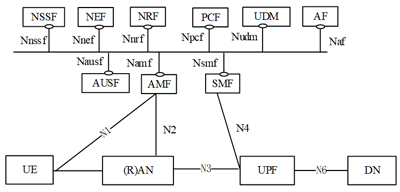
\includegraphics[width=0.8\textwidth]{resources/images/3gpp_5g_system_overview.png}
% 	\caption{3GPP's 5G System Overview \cite{3gpp_5g_system_overview}}
%     \label{fig:introduction:3gpp_5g_system_overview}
% \end{figure}


% \begin{figure}[htbp]
%     \centering
%     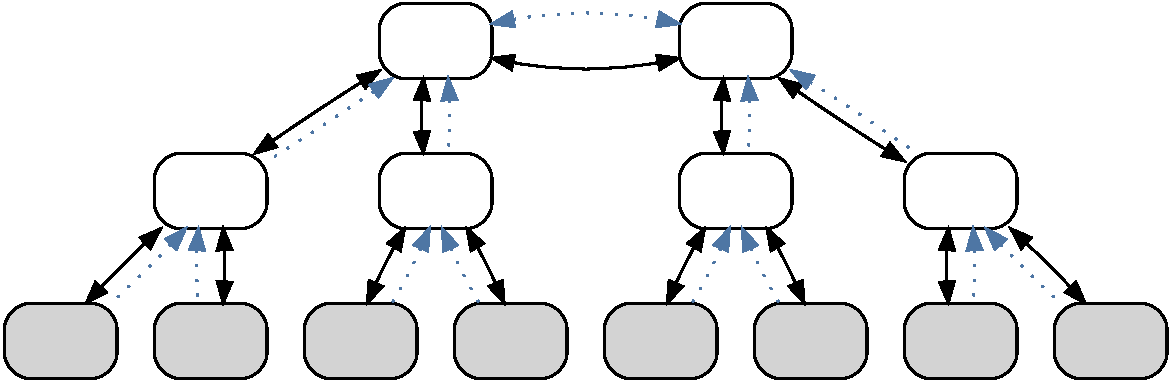
\includegraphics[width=.55\textwidth]{resources/images/example3}
%     \caption{Structure of research}\label{fig:intro:struct}
% \end{figure}

% \sidenote{Research Objectives \& Contributions}
% \todomid{write about the research objectives and \ac{DBpedia} and \Cref{fig:intro:struct}}

% \section{Methodology and Outline}

% \todomid{write about the research outline and \Cref{fig:intro:methodology}. Summarize \Cref{sec:introduction,sec:sota,sec:reqs,sec:contrib1,sec:contrib2,sec:contrib3,sec:eval,sec:summary}.}

% \begin{sidewaysfigure}
%     \centering
%     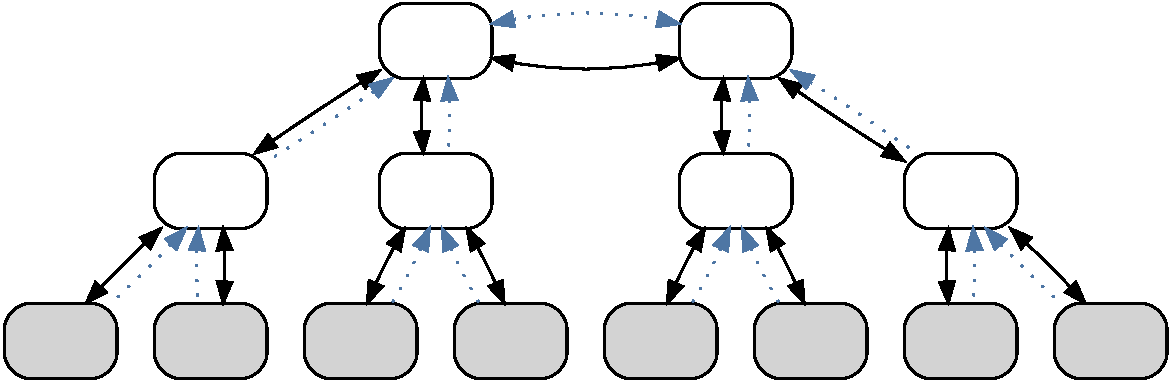
\includegraphics[width=.7\textwidth]{resources/images/example3}
%     \caption{Workflow of the research and structure of the thesis}\label{fig:intro:methodology}
% \end{sidewaysfigure}
